\documentclass[tikz,border=6pt]{standalone}

\usepackage[T1]{fontenc}
\usepackage[utf8]{inputenc}
\usepackage{tikz}
\usetikzlibrary{arrows.meta,positioning,calc,fit,backgrounds}

\definecolor{OccGreen}{RGB}{104,183,120}
\definecolor{DefaultGray}{RGB}{224,224,224}
\definecolor{PathOrange}{RGB}{245,176,65}
\definecolor{PrivateBlue}{RGB}{100,181,246}
\definecolor{PanelGray}{RGB}{248,249,250}

\tikzset{
  node base/.style={
    draw,
    circle,
    minimum size=5.3mm,
    inner sep=0pt,
    font=\scriptsize,
    thick,
  },
  coord node/.style={
    node base,
    fill=white,
    draw=black!60,
  },
  occupied node/.style={
    node base,
    fill=OccGreen!25,
    draw=OccGreen!65!black,
  },
  default node/.style={
    node base,
    fill=DefaultGray,
    draw=gray!65,
    text=gray!70!black,
  },
  target node/.style={
    node base,
    fill=PathOrange!28,
    draw=PathOrange!80!black,
  },
  proof node/.style={
    node base,
    fill=PrivateBlue!24,
    draw=PrivateBlue!75!black,
  },
  panel/.style={
    draw=black!70,
    rounded corners=4pt,
    fill=PanelGray,
    inner sep=5pt,
  },
  note/.style={
    draw,
    rounded corners=2pt,
    fill=white,
    align=left,
    font=\scriptsize,
    inner sep=3pt,
  },
  arrow/.style={-Latex,thick},
}

\begin{document}
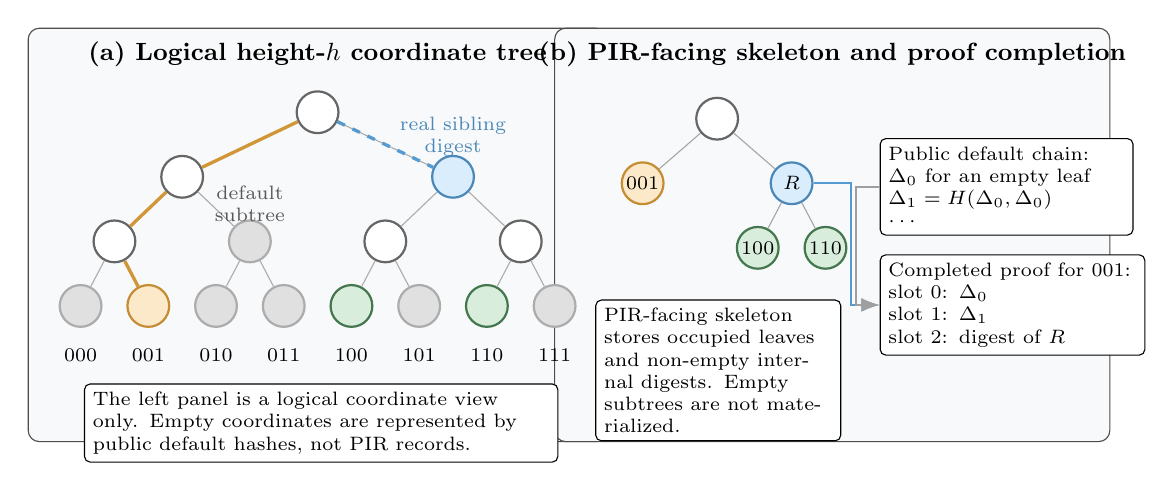
\begin{tikzpicture}[x=0.86cm,y=0.82cm,>=Latex]

\node[font=\bfseries\small] at (2.6,0.45) {(a) Logical height-$h$ coordinate tree};
\node[font=\bfseries\small] at (10.2,0.45) {(b) PIR-facing skeleton and proof completion};

% Logical coordinate tree, h=3.
\node[coord node] (l1) at (2.6,-0.45) {};
\node[coord node] (l2) at (0.6,-1.45) {};
\node[proof node] (l3) at (4.6,-1.45) {};
\node[coord node] (l4) at (-0.4,-2.45) {};
\node[default node] (l5) at (1.6,-2.45) {};
\node[coord node] (l6) at (3.6,-2.45) {};
\node[coord node] (l7) at (5.6,-2.45) {};

\node[default node] (l8) at (-0.9,-3.45) {};
\node[target node] (l9) at (0.1,-3.45) {};
\node[default node] (l10) at (1.1,-3.45) {};
\node[default node] (l11) at (2.1,-3.45) {};
\node[occupied node] (l12) at (3.1,-3.45) {};
\node[default node] (l13) at (4.1,-3.45) {};
\node[occupied node] (l14) at (5.1,-3.45) {};
\node[default node] (l15) at (6.1,-3.45) {};

\foreach \a/\b in {l1/l2,l1/l3,l2/l4,l2/l5,l3/l6,l3/l7,l4/l8,l4/l9,l5/l10,l5/l11,l6/l12,l6/l13,l7/l14,l7/l15}
  \draw[gray!65] (\a) -- (\b);

\draw[PathOrange!85!black,very thick] (l1) -- (l2) -- (l4) -- (l9);
\draw[PrivateBlue!85!black,very thick,dashed] (l1) -- (l3);

\node[font=\scriptsize,below=1.5mm of l8] {$000$};
\node[font=\scriptsize,below=1.5mm of l9] {$001$};
\node[font=\scriptsize,below=1.5mm of l10] {$010$};
\node[font=\scriptsize,below=1.5mm of l11] {$011$};
\node[font=\scriptsize,below=1.5mm of l12] {$100$};
\node[font=\scriptsize,below=1.5mm of l13] {$101$};
\node[font=\scriptsize,below=1.5mm of l14] {$110$};
\node[font=\scriptsize,below=1.5mm of l15] {$111$};

\node[font=\scriptsize,PrivateBlue!75!black,align=center] at ($(l3)+(0.0,0.62)$) {real sibling\\digest};
\node[font=\scriptsize,gray!70!black,align=center] at ($(l5)+(0,0.58)$) {default\\subtree};

% Stored skeleton and completion.
\node[coord node] (s1) at (8.5,-0.55) {};
\node[target node] (s2) at (7.4,-1.55) {$001$};
\node[proof node] (s3) at (9.6,-1.55) {$R$};
\node[occupied node] (s4) at (9.1,-2.55) {$100$};
\node[occupied node] (s5) at (10.1,-2.55) {$110$};

\draw[gray!70] (s1) -- (s2);
\draw[gray!70] (s1) -- (s3);
\draw[gray!70] (s3) -- (s4);
\draw[gray!70] (s3) -- (s5);

\node[note,anchor=north west,text width=2.9cm] (skel) at (6.7,-3.35) {PIR-facing skeleton stores occupied leaves and non-empty internal digests. Empty subtrees are not materialized.};

\node[note,anchor=north west,text width=3.0cm] (defs) at (10.9,-0.85) {Public default chain:\\$\Delta_0$ for an empty leaf\\$\Delta_1=H(\Delta_0,\Delta_0)$\\$\cdots$};

\node[note,anchor=north west,text width=3.15cm] (proof) at (10.9,-2.65) {Completed proof for $001$:\\slot $0$: $\Delta_0$\\slot $1$: $\Delta_1$\\slot $2$: digest of $R$};

\draw[arrow,PrivateBlue!85!black] (s3.east) -- ++(0.55,0) |- (proof.west);
\draw[arrow,gray!75] (defs.west) -- ++(-0.35,0) |- (proof.west);

\node[note,anchor=north west,text width=5.8cm] at (-0.85,-4.65) {The left panel is a logical coordinate view only. Empty coordinates are represented by public default hashes, not PIR records.};

\begin{scope}[on background layer]
  \node[panel,minimum width=7.35cm,minimum height=5.25cm] at (2.6,-2.35) {};
  \node[panel,minimum width=7.05cm,minimum height=5.25cm] at (10.2,-2.35) {};
\end{scope}

\end{tikzpicture}
\end{document}
